% The \phantomsection command is needed to create a link to a place in the document that is not a
% figure, equation, table, section, subsection, chapter, etc.
%
% When do I need to invoke \phantomsection?
% https://tex.stackexchange.com/questions/44088/when-do-i-need-to-invoke-phantomsection
\phantomsection

% ---
\chapter{Proposta e implementação de otimização no PSkel-MPPA}
\label{cap:pskelMPPA}
\phantomsection

\todo[inline]{Praticamente todo o texto que está aqui foi o trabalho do Emmanuel. Logo, isso deve aparecer na seção que explica o PSkel-MPPA. Neste capítulo aqui tu deves explicar o que vai ser modificado (otimizado). Como a comunicação será feita agora? Quais funções da nova API vão ser úteis?}

As otimizações a serem propostas e implementação propriamente dita das mesmas seguirá o modelo mestre-trabalhador, que é um dos padrões de computação paralela que pode ser utilizado quando existem múltiplos núcleos de processamento. O processo mestre é executado no \emph{cluster} de \io conectado a memória LPDDR3, aonde os dados de entrada e saída (os \emph{Array2Ds}) são alocados, enquanto os processos dos trabalhadores são executados nos \emph{clusters} de computação (um processo trabalhador por \emph{cluster} de computação) para realizar a computação estêncil. Devido a memória limitada nos \emph{clusters} de computação (2MB), o tamanho do \emph{Array2D} é particionado em \emph{tiles} de tamanho fixo definido pelo usuário para serem enviados à eles. Quando se trata de particionamento de computação estêncil, é necessário tratar as depedências de vizinhança provenientes do padrão paralelo estêncil, antes de particionar os dados de entrada.

A técnica de \emph{tiling} trapezoidal continuou sendo utilizada para tratar as dependências de vizinhança, o que resulta na computação e presença redundante de dados~\cite{Rocha:2017}. A definição formal está ilustrada a seguir.
Seja $A$ uma matriz de dados 2D, com dimensões $\textrm{dim}(A) = (w, h)$, aonde $w$ e $h$ são, respectivamente, sua largura e altura.
Utilizando \emph{tiles} de dimensões $(w^\prime, h^\prime)$ temos $\lceil\frac{w}{w^\prime}\rceil\lceil\frac{h}{h^\prime}\rceil$ como sendo os possíves \emph{tiles} de $A$.
Seja $A_{i,j}$ um único \emph{tile}, onde $0\leq i < \lceil\frac{w}{ w^\prime}\rceil$ e $0\leq j < \lceil\frac{h}{ h^\prime}\rceil$.
$A_{i,j}$ possui um deslocamento de $(i w^\prime,j h^\prime)$ em relação ao canto superior esquerdo de $A$ e $\textrm{dim}(A_{i,j}) = (\min\{w^\prime, w-i w^\prime\}, \min\{h^\prime, h-j h^\prime\})$.
Esse deslocamento atua como um indexador necessário para acessar os elementos de um \emph{tile}.

A Figura~\ref{fig:gputile} mostra a representação gráfica dessa técnica. Um \emph{tile} lógico (linha contínua interna) está contido em uma matriz de dados 2D (linha pontilhada externa) com deslocamento vertical e horizontal definidos por $j h^\prime$ e $i w^\prime$. Se $t$ iterações de uma aplicação estêncil devem ser executadas, é possível computar $t^\prime$ consecutivas iterações em $A_{i,j}$ ($t^\prime \in \left[1,t\right]$) se precissar de qualquer troca de dados entre \emph{tiles} adjacentes (também conheçido como iterações internas). Assim, o \emph{tile} lógico ($A_{i,j}$) precisa ser engordado, com o acréscimo de uma \emph{ghost zone} (área entre a linha sólida interna e externa), o que inclui a \emph{halo region} (a área entre a linha sólida interna e a linha pontilhada interna). Seja $r$ o mais distante deslocamento necessário para a vizinhança definida pela máscara estêncil. A área de alcance $r$ que define a vizinhança é denominada \textit{halo region}. O número de \emph{halo regions} adjacentes que compõe a \emph{ghost zone} é proporcional a $t^\prime$.
%
Assim, \emph{tile} engordado $A^\ast_{i,j}$ possui deslocamentos $(\max\{iw^\prime - rt^\prime, 0\}, \max\{jh^\prime - rt^\prime, 0\})$ relativos a $A$. Dessa maneira, determinar o tamanho das \emph{ghost zones} implica no \emph{trade-off} entre o custo de computação redundante e a redução de comunicação e sincronização na \noc quando se processa uma computação estêncil iterativa no \mppa.

\begin{figure}[htb]
	\centering
	\caption{Técnica de \textit{tiling} 2D.}
	\includegraphics[width=0.5\textwidth]{figs/tile.pdf} \\
	\legend{Fonte - {\cite{Rocha:2017}}}
	\label{fig:gputile}
\end{figure}

\begin{figure}[htb]
	\centering
	\caption{Comunicações com \texttt{block2d}.}
	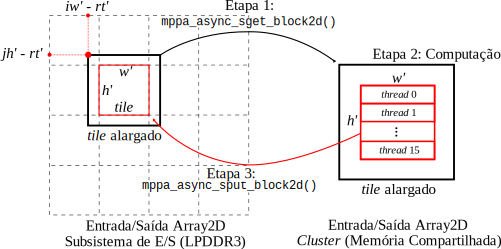
\includegraphics[width=1\textwidth]{figs/pskel-mppa-fluxogram.pdf} \\
	\legend{Fonte - o autor}
    \label{fig:block2d}
\end{figure}

O fluxo de execução do \pskelmppa ocorre da seguinte forma. Durante a fase de inicialização, o processo mestre que está executando no \emph{cluster} de \io aloca os dados de entrada e saída na \lpddr, e cria um segmento específico para cada um deles. Em seguida, ele calcula o número de \emph{tiles} engordados que serão produzidos assim como suas dimensões baseado em: i) parametros definidos pelo usuário, como o tamanho da entrada de dados e as dimensões do \emph{tile} lógico, o número de \emph{clusters} de computação e o número de iterações internas; e ii) parâmetros do \emph{kernel} estêncil, como o tamanho da máscara. Então, são lançados até 16 processos trabalhadores (um em cada \emph{cluster} de computação) e é informado a cada processo trabalhador o número de \emph{tiles} engordados gerados, suas dimensões e o subconjunto de \emph{tiles} que cada \emph{cluster} será responsável por processar. Por fim, o processo mestre aguarda até que todos os trabalhadores terminem de computar.
%
Cada processo trabalhador, por outro lado, aloca dados para armazenar os \emph{tiles} engordados de entrada e de saída na memória local do \emph{cluster} de computação e clona ambos os segmentos de entrada e saída que foram criados pelo processo mestre para realizar futuras transferências de dados. A fase de inicialização tanto do mestre como do trabalhor está encapsulada na classe \texttt{Stencil2D}.
%
Essa primeira etapa do fluxo de execução diferencia-se da anteriormente presente no PSkelMPPA, pois agora esta comunicação é realizada uma única vez na inicialização, o que não ocorria anteriormente, já que exisitiam trocas de mensagens de sincronização a cada laço da computação iterativa.

A fase de computação consiste da execução do \emph{kernel} estêncil pelos processos trabalhadores. As seguintes três principais etapas são realizadas para computar cada \emph{tile} atribuído a um processo trabalhador: 1) o \emph{tile} engordado é extraido do dado de entrada alocado na \lpddr e transferido para a memória local do \emph{cluster} de computação para ser processado; 2) $t^\prime$ iterações do \emph{kernel} estêncil (iterações internas) são executadas pelo processo trabalhor sobre o \emph{tile} engordado; e 3) o \emph{tile} lógico resultante é transferido de volta da memória local do \emph{cluster} de computação para a sua posição correspondente na \lpddr. Assim que todos os \emph{tiles} atribuídos a cada processo trabalhador forem computados com sucesso, todos os processos trabalhadores irão sincronizar em uma barreira global, pois os processos trabalhadores precisarão dos dados computados pelos outros durante as $t^\prime$ iterações para resolverem as dependências de vizinhança das próximas iterações a serem computadas. 
Foi usada a função \texttt{mppa\_rpc\_barrier\_all()} para esse propósito. Todo este processo anteriormente descrito é repetido até que o número total de iterações definido pelo usuário ($t$) seja alcançado.

As etapas acima mencionadas estão retratadas na Figura~\ref{fig:block2d}, para sua implementação foi utilizada uma nova \api de comunicação asíncrona (ASYNC) disponível para o \mppa, que difere da \api anteriormente utilizada, a \ipc. Abaixo elas são descritas em mais detalhes:

\begin{description}

	\item[Etapa 1.] Baseado na informação fornecida pelo processo mestre durante o processo de lançamento dos \emph{clusters} de computação, o processo trabalhador é capaz de calcular as coordenadas de cada \emph{tile} enlargado atribuído a ele em relação aos dados de entrada alocados na \lpddr ($iw^\prime - rt^\prime$ e $jh^\prime - rt^\prime$ coordenadas) sem nenhuma intervenção extra do processo mestre. A função \texttt{mppa\_async\_sget\_block2d()} recebe essa informação e o tamanho do bloco como parâmetros de entrada e ela transfere o \emph{tile} engordado para ser processado pelo processo trabalhador do segmento remoto de entrada para a memória local do \emph{cluster} de computação através da \noc.

	\item[Etapa 2.] O processo trabalhador computa as $t^\prime$ iterações do \emph{kernel} estêncil definido pelo usuário sobre o \emph{tile} engordado. Em cada $t^\prime$ iteração, a computação é paralelizada por meio de uma região paralela de OpenMP. A região paralela cria até 16 \emph{threads} (uma para cada \pe). Cada \pe é responsável por executar o \emph{kernel} estêncil em um subconjunto das células de um \emph{tile} engordado.

	\item[Etapa 3.] Após a computação do \emph{kernel} estêncil, o\emph{tile} lógico resultante é transferido de volta para a \lpddr. A função \texttt{mppa\_async\_sput\_block2d()} é usada para esse propósito, permitindo que o \emph{tile} lógico seja extraído do \emph{tile} engordado na memória local do \emph{cluster} de computação e seja transferido para sua posicão correspondente no segmento de saída remoto.

\end{description}

Felizmente, todas a complexas tarefas relacionas a técnica de \emph{tiling}, comunicação via \noc e adaptações discutidas nessa seção são transparentes para os desenvolvedores, tendo em vista que estão incluidas no \emph{back-end} do PSkelMPPA. Isso significa que aplicações desenvolvidas com o \fw PSkel podem executar perfeitamente no \mppa sem nenhuma alteração no seu código fonte.
